% !TEX encoding = UTF-8 Unicode
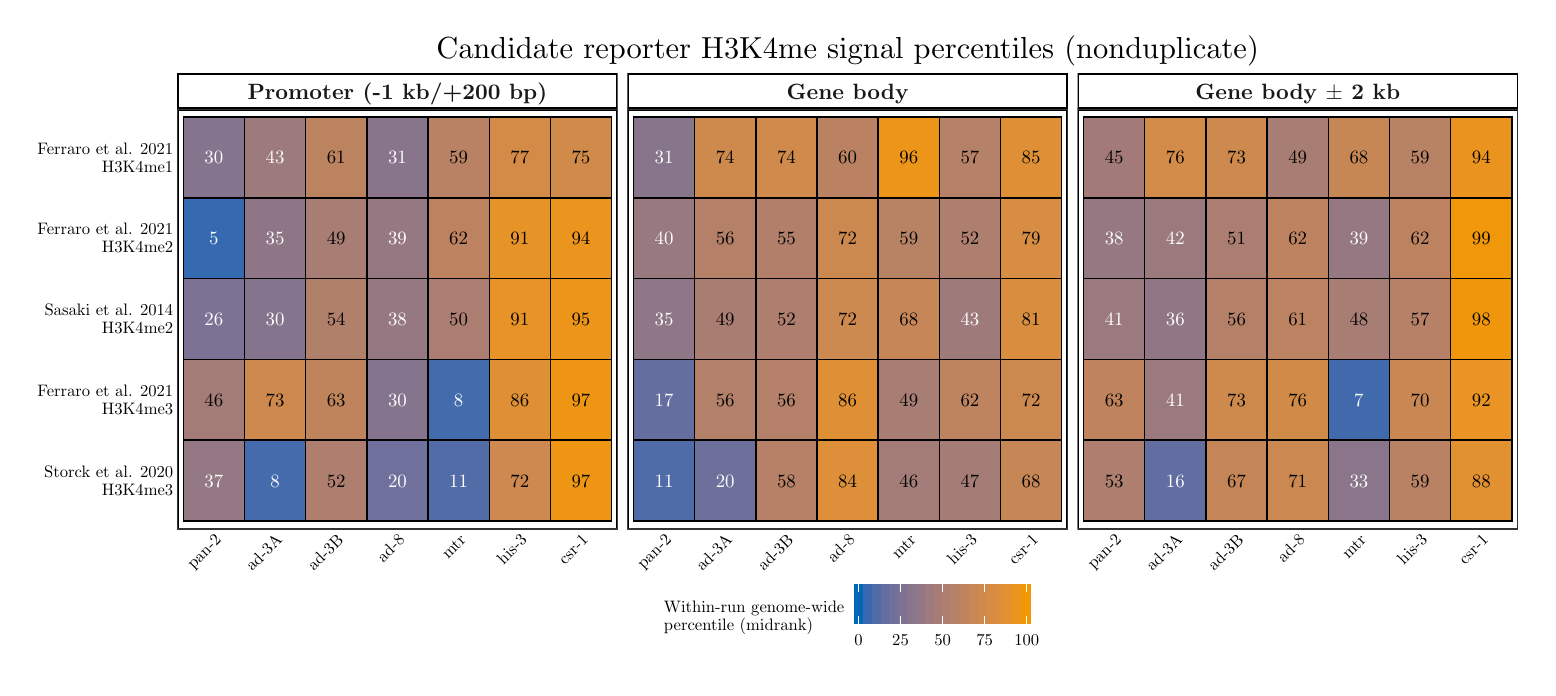
\begin{tikzpicture}[x=1pt,y=1pt]
\definecolor{fillColor}{RGB}{255,255,255}
\path[use as bounding box,fill=fillColor,fill opacity=0.00] (0,0) rectangle (542.02,231.26);
\begin{scope}
\path[clip] (  0.00,  0.00) rectangle (542.02,231.26);
\definecolor{drawColor}{RGB}{255,255,255}
\definecolor{fillColor}{RGB}{255,255,255}

\path[draw=drawColor,line width= 0.7pt,line join=round,line cap=round,fill=fillColor] ( -0.00,  0.00) rectangle (542.02,231.26);
\end{scope}
\begin{scope}
\path[clip] ( 54.02, 50.09) rectangle (213.19,201.87);
\definecolor{drawColor}{RGB}{0,0,0}
\definecolor{fillColor}{RGB}{255,255,255}

\path[draw=drawColor,line width= 1.1pt,line join=round,line cap=round,fill=fillColor] ( 54.02, 50.09) rectangle (213.19,201.87);
\definecolor{fillColor}{RGB}{133,116,141}

\path[draw=drawColor,line width= 0.5pt,fill=fillColor] ( 56.23,169.77) rectangle ( 78.34,198.95);
\definecolor{fillColor}{RGB}{157,122,124}

\path[draw=drawColor,line width= 0.5pt,fill=fillColor] ( 78.34,169.77) rectangle (100.45,198.95);
\definecolor{fillColor}{RGB}{188,131,97}

\path[draw=drawColor,line width= 0.5pt,fill=fillColor] (100.45,169.77) rectangle (122.55,198.95);
\definecolor{fillColor}{RGB}{136,117,140}

\path[draw=drawColor,line width= 0.5pt,fill=fillColor] (122.55,169.77) rectangle (144.66,198.95);
\definecolor{fillColor}{RGB}{185,130,100}

\path[draw=drawColor,line width= 0.5pt,fill=fillColor] (144.66,169.77) rectangle (166.77,198.95);
\definecolor{fillColor}{RGB}{211,139,71}

\path[draw=drawColor,line width= 0.5pt,fill=fillColor] (166.77,169.77) rectangle (188.87,198.95);
\definecolor{fillColor}{RGB}{208,138,74}

\path[draw=drawColor,line width= 0.5pt,fill=fillColor] (188.87,169.77) rectangle (210.98,198.95);
\definecolor{fillColor}{RGB}{53,105,176}

\path[draw=drawColor,line width= 0.5pt,fill=fillColor] ( 56.23,140.58) rectangle ( 78.34,169.77);
\definecolor{fillColor}{RGB}{143,118,135}

\path[draw=drawColor,line width= 0.5pt,fill=fillColor] ( 78.34,140.58) rectangle (100.45,169.77);
\definecolor{fillColor}{RGB}{168,125,115}

\path[draw=drawColor,line width= 0.5pt,fill=fillColor] (100.45,140.58) rectangle (122.55,169.77);
\definecolor{fillColor}{RGB}{150,120,130}

\path[draw=drawColor,line width= 0.5pt,fill=fillColor] (122.55,140.58) rectangle (144.66,169.77);
\definecolor{fillColor}{RGB}{189,131,96}

\path[draw=drawColor,line width= 0.5pt,fill=fillColor] (144.66,140.58) rectangle (166.77,169.77);
\definecolor{fillColor}{RGB}{230,147,40}

\path[draw=drawColor,line width= 0.5pt,fill=fillColor] (166.77,140.58) rectangle (188.87,169.77);
\definecolor{fillColor}{RGB}{235,148,30}

\path[draw=drawColor,line width= 0.5pt,fill=fillColor] (188.87,140.58) rectangle (210.98,169.77);
\definecolor{fillColor}{RGB}{124,114,147}

\path[draw=drawColor,line width= 0.5pt,fill=fillColor] ( 56.23,111.39) rectangle ( 78.34,140.58);
\definecolor{fillColor}{RGB}{133,116,141}

\path[draw=drawColor,line width= 0.5pt,fill=fillColor] ( 78.34,111.39) rectangle (100.45,140.58);
\definecolor{fillColor}{RGB}{177,128,107}

\path[draw=drawColor,line width= 0.5pt,fill=fillColor] (100.45,111.39) rectangle (122.55,140.58);
\definecolor{fillColor}{RGB}{149,120,130}

\path[draw=drawColor,line width= 0.5pt,fill=fillColor] (122.55,111.39) rectangle (144.66,140.58);
\definecolor{fillColor}{RGB}{171,126,113}

\path[draw=drawColor,line width= 0.5pt,fill=fillColor] (144.66,111.39) rectangle (166.77,140.58);
\definecolor{fillColor}{RGB}{231,147,40}

\path[draw=drawColor,line width= 0.5pt,fill=fillColor] (166.77,111.39) rectangle (188.87,140.58);
\definecolor{fillColor}{RGB}{237,149,26}

\path[draw=drawColor,line width= 0.5pt,fill=fillColor] (188.87,111.39) rectangle (210.98,140.58);
\definecolor{fillColor}{RGB}{164,124,119}

\path[draw=drawColor,line width= 0.5pt,fill=fillColor] ( 56.23, 82.20) rectangle ( 78.34,111.39);
\definecolor{fillColor}{RGB}{205,137,78}

\path[draw=drawColor,line width= 0.5pt,fill=fillColor] ( 78.34, 82.20) rectangle (100.45,111.39);
\definecolor{fillColor}{RGB}{192,132,93}

\path[draw=drawColor,line width= 0.5pt,fill=fillColor] (100.45, 82.20) rectangle (122.55,111.39);
\definecolor{fillColor}{RGB}{132,116,142}

\path[draw=drawColor,line width= 0.5pt,fill=fillColor] (122.55, 82.20) rectangle (144.66,111.39);
\definecolor{fillColor}{RGB}{68,107,172}

\path[draw=drawColor,line width= 0.5pt,fill=fillColor] (144.66, 82.20) rectangle (166.77,111.39);
\definecolor{fillColor}{RGB}{223,144,53}

\path[draw=drawColor,line width= 0.5pt,fill=fillColor] (166.77, 82.20) rectangle (188.87,111.39);
\definecolor{fillColor}{RGB}{238,150,19}

\path[draw=drawColor,line width= 0.5pt,fill=fillColor] (188.87, 82.20) rectangle (210.98,111.39);
\definecolor{fillColor}{RGB}{148,120,131}

\path[draw=drawColor,line width= 0.5pt,fill=fillColor] ( 56.23, 53.01) rectangle ( 78.34, 82.20);
\definecolor{fillColor}{RGB}{70,107,172}

\path[draw=drawColor,line width= 0.5pt,fill=fillColor] ( 78.34, 53.01) rectangle (100.45, 82.20);
\definecolor{fillColor}{RGB}{174,127,110}

\path[draw=drawColor,line width= 0.5pt,fill=fillColor] (100.45, 53.01) rectangle (122.55, 82.20);
\definecolor{fillColor}{RGB}{111,112,155}

\path[draw=drawColor,line width= 0.5pt,fill=fillColor] (122.55, 53.01) rectangle (144.66, 82.20);
\definecolor{fillColor}{RGB}{82,108,167}

\path[draw=drawColor,line width= 0.5pt,fill=fillColor] (144.66, 53.01) rectangle (166.77, 82.20);
\definecolor{fillColor}{RGB}{205,137,79}

\path[draw=drawColor,line width= 0.5pt,fill=fillColor] (166.77, 53.01) rectangle (188.87, 82.20);
\definecolor{fillColor}{RGB}{238,150,19}

\path[draw=drawColor,line width= 0.5pt,fill=fillColor] (188.87, 53.01) rectangle (210.98, 82.20);
\definecolor{drawColor}{RGB}{255,255,255}

\node[text=drawColor,anchor=base,inner sep=0pt, outer sep=0pt, scale=  0.68] at ( 67.29,182.01) {30};

\node[text=drawColor,anchor=base,inner sep=0pt, outer sep=0pt, scale=  0.68] at ( 89.39,182.01) {43};
\definecolor{drawColor}{RGB}{0,0,0}

\node[text=drawColor,anchor=base,inner sep=0pt, outer sep=0pt, scale=  0.68] at (111.50,182.01) {61};
\definecolor{drawColor}{RGB}{255,255,255}

\node[text=drawColor,anchor=base,inner sep=0pt, outer sep=0pt, scale=  0.68] at (133.61,182.01) {31};
\definecolor{drawColor}{RGB}{0,0,0}

\node[text=drawColor,anchor=base,inner sep=0pt, outer sep=0pt, scale=  0.68] at (155.71,182.01) {59};

\node[text=drawColor,anchor=base,inner sep=0pt, outer sep=0pt, scale=  0.68] at (177.82,182.01) {77};

\node[text=drawColor,anchor=base,inner sep=0pt, outer sep=0pt, scale=  0.68] at (199.93,182.01) {75};
\definecolor{drawColor}{RGB}{255,255,255}

\node[text=drawColor,anchor=base,inner sep=0pt, outer sep=0pt, scale=  0.68] at ( 67.29,152.82) {5};

\node[text=drawColor,anchor=base,inner sep=0pt, outer sep=0pt, scale=  0.68] at ( 89.39,152.82) {35};
\definecolor{drawColor}{RGB}{0,0,0}

\node[text=drawColor,anchor=base,inner sep=0pt, outer sep=0pt, scale=  0.68] at (111.50,152.82) {49};
\definecolor{drawColor}{RGB}{255,255,255}

\node[text=drawColor,anchor=base,inner sep=0pt, outer sep=0pt, scale=  0.68] at (133.61,152.82) {39};
\definecolor{drawColor}{RGB}{0,0,0}

\node[text=drawColor,anchor=base,inner sep=0pt, outer sep=0pt, scale=  0.68] at (155.71,152.82) {62};

\node[text=drawColor,anchor=base,inner sep=0pt, outer sep=0pt, scale=  0.68] at (177.82,152.82) {91};

\node[text=drawColor,anchor=base,inner sep=0pt, outer sep=0pt, scale=  0.68] at (199.93,152.82) {94};
\definecolor{drawColor}{RGB}{255,255,255}

\node[text=drawColor,anchor=base,inner sep=0pt, outer sep=0pt, scale=  0.68] at ( 67.29,123.63) {26};

\node[text=drawColor,anchor=base,inner sep=0pt, outer sep=0pt, scale=  0.68] at ( 89.39,123.63) {30};
\definecolor{drawColor}{RGB}{0,0,0}

\node[text=drawColor,anchor=base,inner sep=0pt, outer sep=0pt, scale=  0.68] at (111.50,123.63) {54};
\definecolor{drawColor}{RGB}{255,255,255}

\node[text=drawColor,anchor=base,inner sep=0pt, outer sep=0pt, scale=  0.68] at (133.61,123.63) {38};
\definecolor{drawColor}{RGB}{0,0,0}

\node[text=drawColor,anchor=base,inner sep=0pt, outer sep=0pt, scale=  0.68] at (155.71,123.63) {50};

\node[text=drawColor,anchor=base,inner sep=0pt, outer sep=0pt, scale=  0.68] at (177.82,123.63) {91};

\node[text=drawColor,anchor=base,inner sep=0pt, outer sep=0pt, scale=  0.68] at (199.93,123.63) {95};

\node[text=drawColor,anchor=base,inner sep=0pt, outer sep=0pt, scale=  0.68] at ( 67.29, 94.44) {46};

\node[text=drawColor,anchor=base,inner sep=0pt, outer sep=0pt, scale=  0.68] at ( 89.39, 94.44) {73};

\node[text=drawColor,anchor=base,inner sep=0pt, outer sep=0pt, scale=  0.68] at (111.50, 94.44) {63};
\definecolor{drawColor}{RGB}{255,255,255}

\node[text=drawColor,anchor=base,inner sep=0pt, outer sep=0pt, scale=  0.68] at (133.61, 94.44) {30};

\node[text=drawColor,anchor=base,inner sep=0pt, outer sep=0pt, scale=  0.68] at (155.71, 94.44) {8};
\definecolor{drawColor}{RGB}{0,0,0}

\node[text=drawColor,anchor=base,inner sep=0pt, outer sep=0pt, scale=  0.68] at (177.82, 94.44) {86};

\node[text=drawColor,anchor=base,inner sep=0pt, outer sep=0pt, scale=  0.68] at (199.93, 94.44) {97};
\definecolor{drawColor}{RGB}{255,255,255}

\node[text=drawColor,anchor=base,inner sep=0pt, outer sep=0pt, scale=  0.68] at ( 67.29, 65.25) {37};

\node[text=drawColor,anchor=base,inner sep=0pt, outer sep=0pt, scale=  0.68] at ( 89.39, 65.25) {8};
\definecolor{drawColor}{RGB}{0,0,0}

\node[text=drawColor,anchor=base,inner sep=0pt, outer sep=0pt, scale=  0.68] at (111.50, 65.25) {52};
\definecolor{drawColor}{RGB}{255,255,255}

\node[text=drawColor,anchor=base,inner sep=0pt, outer sep=0pt, scale=  0.68] at (133.61, 65.25) {20};

\node[text=drawColor,anchor=base,inner sep=0pt, outer sep=0pt, scale=  0.68] at (155.71, 65.25) {11};
\definecolor{drawColor}{RGB}{0,0,0}

\node[text=drawColor,anchor=base,inner sep=0pt, outer sep=0pt, scale=  0.68] at (177.82, 65.25) {72};

\node[text=drawColor,anchor=base,inner sep=0pt, outer sep=0pt, scale=  0.68] at (199.93, 65.25) {97};
\definecolor{drawColor}{gray}{0.20}

\path[draw=drawColor,line width= 0.7pt,line join=round,line cap=round] ( 54.02, 50.09) rectangle (213.19,201.87);
\end{scope}
\begin{scope}
\path[clip] (216.69, 50.09) rectangle (375.86,201.87);
\definecolor{drawColor}{RGB}{0,0,0}
\definecolor{fillColor}{RGB}{255,255,255}

\path[draw=drawColor,line width= 1.1pt,line join=round,line cap=round,fill=fillColor] (216.69, 50.09) rectangle (375.86,201.87);
\definecolor{fillColor}{RGB}{135,117,140}

\path[draw=drawColor,line width= 0.5pt,fill=fillColor] (218.90,169.77) rectangle (241.01,198.95);
\definecolor{fillColor}{RGB}{206,138,77}

\path[draw=drawColor,line width= 0.5pt,fill=fillColor] (241.01,169.77) rectangle (263.11,198.95);
\definecolor{fillColor}{RGB}{207,138,76}

\path[draw=drawColor,line width= 0.5pt,fill=fillColor] (263.11,169.77) rectangle (285.22,198.95);
\definecolor{fillColor}{RGB}{186,130,99}

\path[draw=drawColor,line width= 0.5pt,fill=fillColor] (285.22,169.77) rectangle (307.33,198.95);
\definecolor{fillColor}{RGB}{237,149,25}

\path[draw=drawColor,line width= 0.5pt,fill=fillColor] (307.33,169.77) rectangle (329.43,198.95);
\definecolor{fillColor}{RGB}{181,129,104}

\path[draw=drawColor,line width= 0.5pt,fill=fillColor] (329.43,169.77) rectangle (351.54,198.95);
\definecolor{fillColor}{RGB}{223,144,54}

\path[draw=drawColor,line width= 0.5pt,fill=fillColor] (351.54,169.77) rectangle (373.65,198.95);
\definecolor{fillColor}{RGB}{152,121,128}

\path[draw=drawColor,line width= 0.5pt,fill=fillColor] (218.90,140.58) rectangle (241.01,169.77);
\definecolor{fillColor}{RGB}{180,129,104}

\path[draw=drawColor,line width= 0.5pt,fill=fillColor] (241.01,140.58) rectangle (263.11,169.77);
\definecolor{fillColor}{RGB}{178,128,106}

\path[draw=drawColor,line width= 0.5pt,fill=fillColor] (263.11,140.58) rectangle (285.22,169.77);
\definecolor{fillColor}{RGB}{204,137,79}

\path[draw=drawColor,line width= 0.5pt,fill=fillColor] (285.22,140.58) rectangle (307.33,169.77);
\definecolor{fillColor}{RGB}{184,130,100}

\path[draw=drawColor,line width= 0.5pt,fill=fillColor] (307.33,140.58) rectangle (329.43,169.77);
\definecolor{fillColor}{RGB}{174,127,110}

\path[draw=drawColor,line width= 0.5pt,fill=fillColor] (329.43,140.58) rectangle (351.54,169.77);
\definecolor{fillColor}{RGB}{215,141,67}

\path[draw=drawColor,line width= 0.5pt,fill=fillColor] (351.54,140.58) rectangle (373.65,169.77);
\definecolor{fillColor}{RGB}{143,119,135}

\path[draw=drawColor,line width= 0.5pt,fill=fillColor] (218.90,111.39) rectangle (241.01,140.58);
\definecolor{fillColor}{RGB}{169,125,114}

\path[draw=drawColor,line width= 0.5pt,fill=fillColor] (241.01,111.39) rectangle (263.11,140.58);
\definecolor{fillColor}{RGB}{174,127,110}

\path[draw=drawColor,line width= 0.5pt,fill=fillColor] (263.11,111.39) rectangle (285.22,140.58);
\definecolor{fillColor}{RGB}{204,137,80}

\path[draw=drawColor,line width= 0.5pt,fill=fillColor] (285.22,111.39) rectangle (307.33,140.58);
\definecolor{fillColor}{RGB}{198,134,87}

\path[draw=drawColor,line width= 0.5pt,fill=fillColor] (307.33,111.39) rectangle (329.43,140.58);
\definecolor{fillColor}{RGB}{159,122,123}

\path[draw=drawColor,line width= 0.5pt,fill=fillColor] (329.43,111.39) rectangle (351.54,140.58);
\definecolor{fillColor}{RGB}{217,142,63}

\path[draw=drawColor,line width= 0.5pt,fill=fillColor] (351.54,111.39) rectangle (373.65,140.58);
\definecolor{fillColor}{RGB}{100,111,160}

\path[draw=drawColor,line width= 0.5pt,fill=fillColor] (218.90, 82.20) rectangle (241.01,111.39);
\definecolor{fillColor}{RGB}{179,128,105}

\path[draw=drawColor,line width= 0.5pt,fill=fillColor] (241.01, 82.20) rectangle (263.11,111.39);
\definecolor{fillColor}{RGB}{180,128,105}

\path[draw=drawColor,line width= 0.5pt,fill=fillColor] (263.11, 82.20) rectangle (285.22,111.39);
\definecolor{fillColor}{RGB}{223,144,53}

\path[draw=drawColor,line width= 0.5pt,fill=fillColor] (285.22, 82.20) rectangle (307.33,111.39);
\definecolor{fillColor}{RGB}{168,125,115}

\path[draw=drawColor,line width= 0.5pt,fill=fillColor] (307.33, 82.20) rectangle (329.43,111.39);
\definecolor{fillColor}{RGB}{190,132,95}

\path[draw=drawColor,line width= 0.5pt,fill=fillColor] (329.43, 82.20) rectangle (351.54,111.39);
\definecolor{fillColor}{RGB}{204,137,79}

\path[draw=drawColor,line width= 0.5pt,fill=fillColor] (351.54, 82.20) rectangle (373.65,111.39);
\definecolor{fillColor}{RGB}{80,108,168}

\path[draw=drawColor,line width= 0.5pt,fill=fillColor] (218.90, 53.01) rectangle (241.01, 82.20);
\definecolor{fillColor}{RGB}{109,112,155}

\path[draw=drawColor,line width= 0.5pt,fill=fillColor] (241.01, 53.01) rectangle (263.11, 82.20);
\definecolor{fillColor}{RGB}{182,129,102}

\path[draw=drawColor,line width= 0.5pt,fill=fillColor] (263.11, 53.01) rectangle (285.22, 82.20);
\definecolor{fillColor}{RGB}{221,143,58}

\path[draw=drawColor,line width= 0.5pt,fill=fillColor] (285.22, 53.01) rectangle (307.33, 82.20);
\definecolor{fillColor}{RGB}{163,124,119}

\path[draw=drawColor,line width= 0.5pt,fill=fillColor] (307.33, 53.01) rectangle (329.43, 82.20);
\definecolor{fillColor}{RGB}{165,124,118}

\path[draw=drawColor,line width= 0.5pt,fill=fillColor] (329.43, 53.01) rectangle (351.54, 82.20);
\definecolor{fillColor}{RGB}{198,134,86}

\path[draw=drawColor,line width= 0.5pt,fill=fillColor] (351.54, 53.01) rectangle (373.65, 82.20);
\definecolor{drawColor}{RGB}{255,255,255}

\node[text=drawColor,anchor=base,inner sep=0pt, outer sep=0pt, scale=  0.68] at (229.95,182.01) {31};
\definecolor{drawColor}{RGB}{0,0,0}

\node[text=drawColor,anchor=base,inner sep=0pt, outer sep=0pt, scale=  0.68] at (252.06,182.01) {74};

\node[text=drawColor,anchor=base,inner sep=0pt, outer sep=0pt, scale=  0.68] at (274.17,182.01) {74};

\node[text=drawColor,anchor=base,inner sep=0pt, outer sep=0pt, scale=  0.68] at (296.27,182.01) {60};

\node[text=drawColor,anchor=base,inner sep=0pt, outer sep=0pt, scale=  0.68] at (318.38,182.01) {96};

\node[text=drawColor,anchor=base,inner sep=0pt, outer sep=0pt, scale=  0.68] at (340.49,182.01) {57};

\node[text=drawColor,anchor=base,inner sep=0pt, outer sep=0pt, scale=  0.68] at (362.59,182.01) {85};
\definecolor{drawColor}{RGB}{255,255,255}

\node[text=drawColor,anchor=base,inner sep=0pt, outer sep=0pt, scale=  0.68] at (229.95,152.82) {40};
\definecolor{drawColor}{RGB}{0,0,0}

\node[text=drawColor,anchor=base,inner sep=0pt, outer sep=0pt, scale=  0.68] at (252.06,152.82) {56};

\node[text=drawColor,anchor=base,inner sep=0pt, outer sep=0pt, scale=  0.68] at (274.17,152.82) {55};

\node[text=drawColor,anchor=base,inner sep=0pt, outer sep=0pt, scale=  0.68] at (296.27,152.82) {72};

\node[text=drawColor,anchor=base,inner sep=0pt, outer sep=0pt, scale=  0.68] at (318.38,152.82) {59};

\node[text=drawColor,anchor=base,inner sep=0pt, outer sep=0pt, scale=  0.68] at (340.49,152.82) {52};

\node[text=drawColor,anchor=base,inner sep=0pt, outer sep=0pt, scale=  0.68] at (362.59,152.82) {79};
\definecolor{drawColor}{RGB}{255,255,255}

\node[text=drawColor,anchor=base,inner sep=0pt, outer sep=0pt, scale=  0.68] at (229.95,123.63) {35};
\definecolor{drawColor}{RGB}{0,0,0}

\node[text=drawColor,anchor=base,inner sep=0pt, outer sep=0pt, scale=  0.68] at (252.06,123.63) {49};

\node[text=drawColor,anchor=base,inner sep=0pt, outer sep=0pt, scale=  0.68] at (274.17,123.63) {52};

\node[text=drawColor,anchor=base,inner sep=0pt, outer sep=0pt, scale=  0.68] at (296.27,123.63) {72};

\node[text=drawColor,anchor=base,inner sep=0pt, outer sep=0pt, scale=  0.68] at (318.38,123.63) {68};
\definecolor{drawColor}{RGB}{255,255,255}

\node[text=drawColor,anchor=base,inner sep=0pt, outer sep=0pt, scale=  0.68] at (340.49,123.63) {43};
\definecolor{drawColor}{RGB}{0,0,0}

\node[text=drawColor,anchor=base,inner sep=0pt, outer sep=0pt, scale=  0.68] at (362.59,123.63) {81};
\definecolor{drawColor}{RGB}{255,255,255}

\node[text=drawColor,anchor=base,inner sep=0pt, outer sep=0pt, scale=  0.68] at (229.95, 94.44) {17};
\definecolor{drawColor}{RGB}{0,0,0}

\node[text=drawColor,anchor=base,inner sep=0pt, outer sep=0pt, scale=  0.68] at (252.06, 94.44) {56};

\node[text=drawColor,anchor=base,inner sep=0pt, outer sep=0pt, scale=  0.68] at (274.17, 94.44) {56};

\node[text=drawColor,anchor=base,inner sep=0pt, outer sep=0pt, scale=  0.68] at (296.27, 94.44) {86};

\node[text=drawColor,anchor=base,inner sep=0pt, outer sep=0pt, scale=  0.68] at (318.38, 94.44) {49};

\node[text=drawColor,anchor=base,inner sep=0pt, outer sep=0pt, scale=  0.68] at (340.49, 94.44) {62};

\node[text=drawColor,anchor=base,inner sep=0pt, outer sep=0pt, scale=  0.68] at (362.59, 94.44) {72};
\definecolor{drawColor}{RGB}{255,255,255}

\node[text=drawColor,anchor=base,inner sep=0pt, outer sep=0pt, scale=  0.68] at (229.95, 65.25) {11};

\node[text=drawColor,anchor=base,inner sep=0pt, outer sep=0pt, scale=  0.68] at (252.06, 65.25) {20};
\definecolor{drawColor}{RGB}{0,0,0}

\node[text=drawColor,anchor=base,inner sep=0pt, outer sep=0pt, scale=  0.68] at (274.17, 65.25) {58};

\node[text=drawColor,anchor=base,inner sep=0pt, outer sep=0pt, scale=  0.68] at (296.27, 65.25) {84};

\node[text=drawColor,anchor=base,inner sep=0pt, outer sep=0pt, scale=  0.68] at (318.38, 65.25) {46};

\node[text=drawColor,anchor=base,inner sep=0pt, outer sep=0pt, scale=  0.68] at (340.49, 65.25) {47};

\node[text=drawColor,anchor=base,inner sep=0pt, outer sep=0pt, scale=  0.68] at (362.59, 65.25) {68};
\definecolor{drawColor}{gray}{0.20}

\path[draw=drawColor,line width= 0.7pt,line join=round,line cap=round] (216.69, 50.09) rectangle (375.86,201.87);
\end{scope}
\begin{scope}
\path[clip] (379.36, 50.09) rectangle (538.52,201.87);
\definecolor{drawColor}{RGB}{0,0,0}
\definecolor{fillColor}{RGB}{255,255,255}

\path[draw=drawColor,line width= 1.1pt,line join=round,line cap=round,fill=fillColor] (379.36, 50.09) rectangle (538.53,201.87);
\definecolor{fillColor}{RGB}{162,123,120}

\path[draw=drawColor,line width= 0.5pt,fill=fillColor] (381.57,169.77) rectangle (403.67,198.95);
\definecolor{fillColor}{RGB}{210,139,72}

\path[draw=drawColor,line width= 0.5pt,fill=fillColor] (403.67,169.77) rectangle (425.78,198.95);
\definecolor{fillColor}{RGB}{205,137,78}

\path[draw=drawColor,line width= 0.5pt,fill=fillColor] (425.78,169.77) rectangle (447.89,198.95);
\definecolor{fillColor}{RGB}{168,125,115}

\path[draw=drawColor,line width= 0.5pt,fill=fillColor] (447.89,169.77) rectangle (469.99,198.95);
\definecolor{fillColor}{RGB}{199,135,85}

\path[draw=drawColor,line width= 0.5pt,fill=fillColor] (469.99,169.77) rectangle (492.10,198.95);
\definecolor{fillColor}{RGB}{184,130,101}

\path[draw=drawColor,line width= 0.5pt,fill=fillColor] (492.10,169.77) rectangle (514.21,198.95);
\definecolor{fillColor}{RGB}{234,148,31}

\path[draw=drawColor,line width= 0.5pt,fill=fillColor] (514.21,169.77) rectangle (536.31,198.95);
\definecolor{fillColor}{RGB}{150,120,130}

\path[draw=drawColor,line width= 0.5pt,fill=fillColor] (381.57,140.58) rectangle (403.67,169.77);
\definecolor{fillColor}{RGB}{155,122,126}

\path[draw=drawColor,line width= 0.5pt,fill=fillColor] (403.67,140.58) rectangle (425.78,169.77);
\definecolor{fillColor}{RGB}{171,126,113}

\path[draw=drawColor,line width= 0.5pt,fill=fillColor] (425.78,140.58) rectangle (447.89,169.77);
\definecolor{fillColor}{RGB}{189,131,96}

\path[draw=drawColor,line width= 0.5pt,fill=fillColor] (447.89,140.58) rectangle (469.99,169.77);
\definecolor{fillColor}{RGB}{150,120,130}

\path[draw=drawColor,line width= 0.5pt,fill=fillColor] (469.99,140.58) rectangle (492.10,169.77);
\definecolor{fillColor}{RGB}{189,131,96}

\path[draw=drawColor,line width= 0.5pt,fill=fillColor] (492.10,140.58) rectangle (514.21,169.77);
\definecolor{fillColor}{RGB}{241,151,10}

\path[draw=drawColor,line width= 0.5pt,fill=fillColor] (514.21,140.58) rectangle (536.31,169.77);
\definecolor{fillColor}{RGB}{154,121,127}

\path[draw=drawColor,line width= 0.5pt,fill=fillColor] (381.57,111.39) rectangle (403.67,140.58);
\definecolor{fillColor}{RGB}{145,119,134}

\path[draw=drawColor,line width= 0.5pt,fill=fillColor] (403.67,111.39) rectangle (425.78,140.58);
\definecolor{fillColor}{RGB}{180,129,104}

\path[draw=drawColor,line width= 0.5pt,fill=fillColor] (425.78,111.39) rectangle (447.89,140.58);
\definecolor{fillColor}{RGB}{187,131,98}

\path[draw=drawColor,line width= 0.5pt,fill=fillColor] (447.89,111.39) rectangle (469.99,140.58);
\definecolor{fillColor}{RGB}{167,125,116}

\path[draw=drawColor,line width= 0.5pt,fill=fillColor] (469.99,111.39) rectangle (492.10,140.58);
\definecolor{fillColor}{RGB}{182,129,103}

\path[draw=drawColor,line width= 0.5pt,fill=fillColor] (492.10,111.39) rectangle (514.21,140.58);
\definecolor{fillColor}{RGB}{240,150,12}

\path[draw=drawColor,line width= 0.5pt,fill=fillColor] (514.21,111.39) rectangle (536.31,140.58);
\definecolor{fillColor}{RGB}{191,132,94}

\path[draw=drawColor,line width= 0.5pt,fill=fillColor] (381.57, 82.20) rectangle (403.67,111.39);
\definecolor{fillColor}{RGB}{154,121,127}

\path[draw=drawColor,line width= 0.5pt,fill=fillColor] (403.67, 82.20) rectangle (425.78,111.39);
\definecolor{fillColor}{RGB}{206,138,77}

\path[draw=drawColor,line width= 0.5pt,fill=fillColor] (425.78, 82.20) rectangle (447.89,111.39);
\definecolor{fillColor}{RGB}{209,139,73}

\path[draw=drawColor,line width= 0.5pt,fill=fillColor] (447.89, 82.20) rectangle (469.99,111.39);
\definecolor{fillColor}{RGB}{65,106,173}

\path[draw=drawColor,line width= 0.5pt,fill=fillColor] (469.99, 82.20) rectangle (492.10,111.39);
\definecolor{fillColor}{RGB}{201,136,83}

\path[draw=drawColor,line width= 0.5pt,fill=fillColor] (492.10, 82.20) rectangle (514.21,111.39);
\definecolor{fillColor}{RGB}{233,148,37}

\path[draw=drawColor,line width= 0.5pt,fill=fillColor] (514.21, 82.20) rectangle (536.31,111.39);
\definecolor{fillColor}{RGB}{174,127,110}

\path[draw=drawColor,line width= 0.5pt,fill=fillColor] (381.57, 53.01) rectangle (403.67, 82.20);
\definecolor{fillColor}{RGB}{98,110,161}

\path[draw=drawColor,line width= 0.5pt,fill=fillColor] (403.67, 53.01) rectangle (425.78, 82.20);
\definecolor{fillColor}{RGB}{196,134,88}

\path[draw=drawColor,line width= 0.5pt,fill=fillColor] (425.78, 53.01) rectangle (447.89, 82.20);
\definecolor{fillColor}{RGB}{203,137,81}

\path[draw=drawColor,line width= 0.5pt,fill=fillColor] (447.89, 53.01) rectangle (469.99, 82.20);
\definecolor{fillColor}{RGB}{139,117,138}

\path[draw=drawColor,line width= 0.5pt,fill=fillColor] (469.99, 53.01) rectangle (492.10, 82.20);
\definecolor{fillColor}{RGB}{185,130,100}

\path[draw=drawColor,line width= 0.5pt,fill=fillColor] (492.10, 53.01) rectangle (514.21, 82.20);
\definecolor{fillColor}{RGB}{226,145,49}

\path[draw=drawColor,line width= 0.5pt,fill=fillColor] (514.21, 53.01) rectangle (536.31, 82.20);

\node[text=drawColor,anchor=base,inner sep=0pt, outer sep=0pt, scale=  0.68] at (392.62,182.01) {45};

\node[text=drawColor,anchor=base,inner sep=0pt, outer sep=0pt, scale=  0.68] at (414.73,182.01) {76};

\node[text=drawColor,anchor=base,inner sep=0pt, outer sep=0pt, scale=  0.68] at (436.83,182.01) {73};

\node[text=drawColor,anchor=base,inner sep=0pt, outer sep=0pt, scale=  0.68] at (458.94,182.01) {49};

\node[text=drawColor,anchor=base,inner sep=0pt, outer sep=0pt, scale=  0.68] at (481.05,182.01) {68};

\node[text=drawColor,anchor=base,inner sep=0pt, outer sep=0pt, scale=  0.68] at (503.15,182.01) {59};

\node[text=drawColor,anchor=base,inner sep=0pt, outer sep=0pt, scale=  0.68] at (525.26,182.01) {94};
\definecolor{drawColor}{RGB}{255,255,255}

\node[text=drawColor,anchor=base,inner sep=0pt, outer sep=0pt, scale=  0.68] at (392.62,152.82) {38};

\node[text=drawColor,anchor=base,inner sep=0pt, outer sep=0pt, scale=  0.68] at (414.73,152.82) {42};
\definecolor{drawColor}{RGB}{0,0,0}

\node[text=drawColor,anchor=base,inner sep=0pt, outer sep=0pt, scale=  0.68] at (436.83,152.82) {51};

\node[text=drawColor,anchor=base,inner sep=0pt, outer sep=0pt, scale=  0.68] at (458.94,152.82) {62};
\definecolor{drawColor}{RGB}{255,255,255}

\node[text=drawColor,anchor=base,inner sep=0pt, outer sep=0pt, scale=  0.68] at (481.05,152.82) {39};
\definecolor{drawColor}{RGB}{0,0,0}

\node[text=drawColor,anchor=base,inner sep=0pt, outer sep=0pt, scale=  0.68] at (503.15,152.82) {62};

\node[text=drawColor,anchor=base,inner sep=0pt, outer sep=0pt, scale=  0.68] at (525.26,152.82) {99};
\definecolor{drawColor}{RGB}{255,255,255}

\node[text=drawColor,anchor=base,inner sep=0pt, outer sep=0pt, scale=  0.68] at (392.62,123.63) {41};

\node[text=drawColor,anchor=base,inner sep=0pt, outer sep=0pt, scale=  0.68] at (414.73,123.63) {36};
\definecolor{drawColor}{RGB}{0,0,0}

\node[text=drawColor,anchor=base,inner sep=0pt, outer sep=0pt, scale=  0.68] at (436.83,123.63) {56};

\node[text=drawColor,anchor=base,inner sep=0pt, outer sep=0pt, scale=  0.68] at (458.94,123.63) {61};

\node[text=drawColor,anchor=base,inner sep=0pt, outer sep=0pt, scale=  0.68] at (481.05,123.63) {48};

\node[text=drawColor,anchor=base,inner sep=0pt, outer sep=0pt, scale=  0.68] at (503.15,123.63) {57};

\node[text=drawColor,anchor=base,inner sep=0pt, outer sep=0pt, scale=  0.68] at (525.26,123.63) {98};

\node[text=drawColor,anchor=base,inner sep=0pt, outer sep=0pt, scale=  0.68] at (392.62, 94.44) {63};
\definecolor{drawColor}{RGB}{255,255,255}

\node[text=drawColor,anchor=base,inner sep=0pt, outer sep=0pt, scale=  0.68] at (414.73, 94.44) {41};
\definecolor{drawColor}{RGB}{0,0,0}

\node[text=drawColor,anchor=base,inner sep=0pt, outer sep=0pt, scale=  0.68] at (436.83, 94.44) {73};

\node[text=drawColor,anchor=base,inner sep=0pt, outer sep=0pt, scale=  0.68] at (458.94, 94.44) {76};
\definecolor{drawColor}{RGB}{255,255,255}

\node[text=drawColor,anchor=base,inner sep=0pt, outer sep=0pt, scale=  0.68] at (481.05, 94.44) {7};
\definecolor{drawColor}{RGB}{0,0,0}

\node[text=drawColor,anchor=base,inner sep=0pt, outer sep=0pt, scale=  0.68] at (503.15, 94.44) {70};

\node[text=drawColor,anchor=base,inner sep=0pt, outer sep=0pt, scale=  0.68] at (525.26, 94.44) {92};

\node[text=drawColor,anchor=base,inner sep=0pt, outer sep=0pt, scale=  0.68] at (392.62, 65.25) {53};
\definecolor{drawColor}{RGB}{255,255,255}

\node[text=drawColor,anchor=base,inner sep=0pt, outer sep=0pt, scale=  0.68] at (414.73, 65.25) {16};
\definecolor{drawColor}{RGB}{0,0,0}

\node[text=drawColor,anchor=base,inner sep=0pt, outer sep=0pt, scale=  0.68] at (436.83, 65.25) {67};

\node[text=drawColor,anchor=base,inner sep=0pt, outer sep=0pt, scale=  0.68] at (458.94, 65.25) {71};
\definecolor{drawColor}{RGB}{255,255,255}

\node[text=drawColor,anchor=base,inner sep=0pt, outer sep=0pt, scale=  0.68] at (481.05, 65.25) {33};
\definecolor{drawColor}{RGB}{0,0,0}

\node[text=drawColor,anchor=base,inner sep=0pt, outer sep=0pt, scale=  0.68] at (503.15, 65.25) {59};

\node[text=drawColor,anchor=base,inner sep=0pt, outer sep=0pt, scale=  0.68] at (525.26, 65.25) {88};
\definecolor{drawColor}{gray}{0.20}

\path[draw=drawColor,line width= 0.7pt,line join=round,line cap=round] (379.36, 50.09) rectangle (538.53,201.87);
\end{scope}
\begin{scope}
\path[clip] ( 54.02,201.87) rectangle (213.19,214.55);
\definecolor{drawColor}{RGB}{0,0,0}
\definecolor{fillColor}{RGB}{255,255,255}

\path[draw=drawColor,line width= 1.1pt,line join=round,line cap=round,fill=fillColor] ( 54.02,201.87) rectangle (213.19,214.55);
\definecolor{drawColor}{gray}{0.10}

\node[text=drawColor,anchor=base,inner sep=0pt, outer sep=0pt, scale=  0.80] at (133.61,205.45) {\bfseries Promoter (-1 kb/+200 bp)};
\end{scope}
\begin{scope}
\path[clip] (216.69,201.87) rectangle (375.86,214.55);
\definecolor{drawColor}{RGB}{0,0,0}
\definecolor{fillColor}{RGB}{255,255,255}

\path[draw=drawColor,line width= 1.1pt,line join=round,line cap=round,fill=fillColor] (216.69,201.87) rectangle (375.86,214.55);
\definecolor{drawColor}{gray}{0.10}

\node[text=drawColor,anchor=base,inner sep=0pt, outer sep=0pt, scale=  0.80] at (296.27,205.45) {\bfseries Gene body};
\end{scope}
\begin{scope}
\path[clip] (379.36,201.87) rectangle (538.52,214.55);
\definecolor{drawColor}{RGB}{0,0,0}
\definecolor{fillColor}{RGB}{255,255,255}

\path[draw=drawColor,line width= 1.1pt,line join=round,line cap=round,fill=fillColor] (379.36,201.87) rectangle (538.53,214.55);
\definecolor{drawColor}{gray}{0.10}

\node[text=drawColor,anchor=base,inner sep=0pt, outer sep=0pt, scale=  0.80] at (458.94,205.45) {\bfseries Gene body $\pm$ 2 kb};
\end{scope}
\begin{scope}
\path[clip] (  0.00,  0.00) rectangle (542.02,231.26);
\definecolor{drawColor}{RGB}{0,0,0}

\node[text=drawColor,rotate= 45.00,anchor=base east,inner sep=0pt, outer sep=0pt, scale=  0.60] at ( 70.21, 45.77) {pan-2};

\node[text=drawColor,rotate= 45.00,anchor=base east,inner sep=0pt, outer sep=0pt, scale=  0.60] at ( 92.31, 45.77) {ad-3A};

\node[text=drawColor,rotate= 45.00,anchor=base east,inner sep=0pt, outer sep=0pt, scale=  0.60] at (114.42, 45.77) {ad-3B};

\node[text=drawColor,rotate= 45.00,anchor=base east,inner sep=0pt, outer sep=0pt, scale=  0.60] at (136.53, 45.77) {ad-8};

\node[text=drawColor,rotate= 45.00,anchor=base east,inner sep=0pt, outer sep=0pt, scale=  0.60] at (158.63, 45.77) {mtr};

\node[text=drawColor,rotate= 45.00,anchor=base east,inner sep=0pt, outer sep=0pt, scale=  0.60] at (180.74, 45.77) {his-3};

\node[text=drawColor,rotate= 45.00,anchor=base east,inner sep=0pt, outer sep=0pt, scale=  0.60] at (202.85, 45.77) {csr-1};
\end{scope}
\begin{scope}
\path[clip] (  0.00,  0.00) rectangle (542.02,231.26);
\definecolor{drawColor}{RGB}{0,0,0}

\node[text=drawColor,rotate= 45.00,anchor=base east,inner sep=0pt, outer sep=0pt, scale=  0.60] at (232.88, 45.77) {pan-2};

\node[text=drawColor,rotate= 45.00,anchor=base east,inner sep=0pt, outer sep=0pt, scale=  0.60] at (254.98, 45.77) {ad-3A};

\node[text=drawColor,rotate= 45.00,anchor=base east,inner sep=0pt, outer sep=0pt, scale=  0.60] at (277.09, 45.77) {ad-3B};

\node[text=drawColor,rotate= 45.00,anchor=base east,inner sep=0pt, outer sep=0pt, scale=  0.60] at (299.20, 45.77) {ad-8};

\node[text=drawColor,rotate= 45.00,anchor=base east,inner sep=0pt, outer sep=0pt, scale=  0.60] at (321.30, 45.77) {mtr};

\node[text=drawColor,rotate= 45.00,anchor=base east,inner sep=0pt, outer sep=0pt, scale=  0.60] at (343.41, 45.77) {his-3};

\node[text=drawColor,rotate= 45.00,anchor=base east,inner sep=0pt, outer sep=0pt, scale=  0.60] at (365.52, 45.77) {csr-1};
\end{scope}
\begin{scope}
\path[clip] (  0.00,  0.00) rectangle (542.02,231.26);
\definecolor{drawColor}{RGB}{0,0,0}

\node[text=drawColor,rotate= 45.00,anchor=base east,inner sep=0pt, outer sep=0pt, scale=  0.60] at (395.54, 45.77) {pan-2};

\node[text=drawColor,rotate= 45.00,anchor=base east,inner sep=0pt, outer sep=0pt, scale=  0.60] at (417.65, 45.77) {ad-3A};

\node[text=drawColor,rotate= 45.00,anchor=base east,inner sep=0pt, outer sep=0pt, scale=  0.60] at (439.76, 45.77) {ad-3B};

\node[text=drawColor,rotate= 45.00,anchor=base east,inner sep=0pt, outer sep=0pt, scale=  0.60] at (461.86, 45.77) {ad-8};

\node[text=drawColor,rotate= 45.00,anchor=base east,inner sep=0pt, outer sep=0pt, scale=  0.60] at (483.97, 45.77) {mtr};

\node[text=drawColor,rotate= 45.00,anchor=base east,inner sep=0pt, outer sep=0pt, scale=  0.60] at (506.08, 45.77) {his-3};

\node[text=drawColor,rotate= 45.00,anchor=base east,inner sep=0pt, outer sep=0pt, scale=  0.60] at (528.18, 45.77) {csr-1};
\end{scope}
\begin{scope}
\path[clip] (  0.00,  0.00) rectangle (542.02,231.26);
\definecolor{drawColor}{RGB}{0,0,0}

\node[text=drawColor,anchor=base east,inner sep=0pt, outer sep=0pt, scale=  0.60] at ( 52.62, 68.78) {Storck et al. 2020};

\node[text=drawColor,anchor=base east,inner sep=0pt, outer sep=0pt, scale=  0.60] at ( 52.62, 62.30) {H3K4me3};

\node[text=drawColor,anchor=base east,inner sep=0pt, outer sep=0pt, scale=  0.60] at ( 52.62, 97.97) {Ferraro et al. 2021};

\node[text=drawColor,anchor=base east,inner sep=0pt, outer sep=0pt, scale=  0.60] at ( 52.62, 91.49) {H3K4me3};

\node[text=drawColor,anchor=base east,inner sep=0pt, outer sep=0pt, scale=  0.60] at ( 52.62,127.16) {Sasaki et al. 2014};

\node[text=drawColor,anchor=base east,inner sep=0pt, outer sep=0pt, scale=  0.60] at ( 52.62,120.68) {H3K4me2};

\node[text=drawColor,anchor=base east,inner sep=0pt, outer sep=0pt, scale=  0.60] at ( 52.62,156.35) {Ferraro et al. 2021};

\node[text=drawColor,anchor=base east,inner sep=0pt, outer sep=0pt, scale=  0.60] at ( 52.62,149.87) {H3K4me2};

\node[text=drawColor,anchor=base east,inner sep=0pt, outer sep=0pt, scale=  0.60] at ( 52.62,185.53) {Ferraro et al. 2021};

\node[text=drawColor,anchor=base east,inner sep=0pt, outer sep=0pt, scale=  0.60] at ( 52.62,179.05) {H3K4me1};
\end{scope}
\begin{scope}
\path[clip] (  0.00,  0.00) rectangle (542.02,231.26);
\definecolor{fillColor}{RGB}{255,255,255}

\path[fill=fillColor] (226.43,  3.50) rectangle (366.12, 33.75);
\end{scope}
\begin{scope}
\path[clip] (  0.00,  0.00) rectangle (542.02,231.26);
\definecolor{drawColor}{RGB}{0,0,0}

\node[text=drawColor,anchor=base west,inner sep=0pt, outer sep=0pt, scale=  0.60] at (229.93, 19.80) {Within-run genome-wide};

\node[text=drawColor,anchor=base west,inner sep=0pt, outer sep=0pt, scale=  0.60] at (229.93, 13.32) {percentile (midrank)};
\end{scope}
\begin{scope}
\path[clip] (  0.00,  0.00) rectangle (542.02,231.26);
\definecolor{fillColor}{RGB}{0,103,183}

\path[fill=fillColor] (298.60, 15.80) rectangle (301.80, 30.25);
\definecolor{fillColor}{RGB}{56,105,176}

\path[fill=fillColor] (301.80, 15.80) rectangle (305.00, 30.25);
\definecolor{fillColor}{RGB}{80,108,168}

\path[fill=fillColor] (305.00, 15.80) rectangle (308.20, 30.25);
\definecolor{fillColor}{RGB}{98,110,161}

\path[fill=fillColor] (308.20, 15.80) rectangle (311.40, 30.25);
\definecolor{fillColor}{RGB}{112,112,154}

\path[fill=fillColor] (311.40, 15.80) rectangle (314.60, 30.25);
\definecolor{fillColor}{RGB}{125,114,147}

\path[fill=fillColor] (314.60, 15.80) rectangle (317.80, 30.25);
\definecolor{fillColor}{RGB}{137,117,140}

\path[fill=fillColor] (317.80, 15.80) rectangle (321.00, 30.25);
\definecolor{fillColor}{RGB}{147,119,132}

\path[fill=fillColor] (321.00, 15.80) rectangle (324.21, 30.25);
\definecolor{fillColor}{RGB}{156,122,125}

\path[fill=fillColor] (324.21, 15.80) rectangle (327.41, 30.25);
\definecolor{fillColor}{RGB}{166,124,117}

\path[fill=fillColor] (327.41, 15.80) rectangle (330.61, 30.25);
\definecolor{fillColor}{RGB}{174,127,110}

\path[fill=fillColor] (330.61, 15.80) rectangle (333.81, 30.25);
\definecolor{fillColor}{RGB}{183,129,102}

\path[fill=fillColor] (333.81, 15.80) rectangle (337.01, 30.25);
\definecolor{fillColor}{RGB}{191,132,94}

\path[fill=fillColor] (337.01, 15.80) rectangle (340.21, 30.25);
\definecolor{fillColor}{RGB}{199,135,86}

\path[fill=fillColor] (340.21, 15.80) rectangle (343.41, 30.25);
\definecolor{fillColor}{RGB}{206,138,77}

\path[fill=fillColor] (343.41, 15.80) rectangle (346.61, 30.25);
\definecolor{fillColor}{RGB}{214,140,68}

\path[fill=fillColor] (346.61, 15.80) rectangle (349.81, 30.25);
\definecolor{fillColor}{RGB}{221,143,57}

\path[fill=fillColor] (349.81, 15.80) rectangle (353.01, 30.25);
\definecolor{fillColor}{RGB}{229,146,45}

\path[fill=fillColor] (353.01, 15.80) rectangle (356.21, 30.25);
\definecolor{fillColor}{RGB}{236,149,29}

\path[fill=fillColor] (356.21, 15.80) rectangle (359.42, 30.25);
\definecolor{fillColor}{RGB}{242,152,0}

\path[fill=fillColor] (359.42, 15.80) rectangle (362.62, 30.25);
\end{scope}
\begin{scope}
\path[clip] (  0.00,  0.00) rectangle (542.02,231.26);
\definecolor{drawColor}{RGB}{255,255,255}

\path[draw=drawColor,line width= 0.4pt,line join=round] (300.20, 18.69) --
	(300.20, 15.80);

\path[draw=drawColor,line width= 0.4pt,line join=round] (315.40, 18.69) --
	(315.40, 15.80);

\path[draw=drawColor,line width= 0.4pt,line join=round] (330.61, 18.69) --
	(330.61, 15.80);

\path[draw=drawColor,line width= 0.4pt,line join=round] (345.81, 18.69) --
	(345.81, 15.80);

\path[draw=drawColor,line width= 0.4pt,line join=round] (361.02, 18.69) --
	(361.02, 15.80);

\path[draw=drawColor,line width= 0.4pt,line join=round] (300.20, 27.36) --
	(300.20, 30.25);

\path[draw=drawColor,line width= 0.4pt,line join=round] (315.40, 27.36) --
	(315.40, 30.25);

\path[draw=drawColor,line width= 0.4pt,line join=round] (330.61, 27.36) --
	(330.61, 30.25);

\path[draw=drawColor,line width= 0.4pt,line join=round] (345.81, 27.36) --
	(345.81, 30.25);

\path[draw=drawColor,line width= 0.4pt,line join=round] (361.02, 27.36) --
	(361.02, 30.25);
\end{scope}
\begin{scope}
\path[clip] (  0.00,  0.00) rectangle (542.02,231.26);
\definecolor{drawColor}{RGB}{0,0,0}

\node[text=drawColor,anchor=base,inner sep=0pt, outer sep=0pt, scale=  0.60] at (300.20,  8.17) {0};

\node[text=drawColor,anchor=base,inner sep=0pt, outer sep=0pt, scale=  0.60] at (315.40,  8.17) {25};

\node[text=drawColor,anchor=base,inner sep=0pt, outer sep=0pt, scale=  0.60] at (330.61,  8.17) {50};

\node[text=drawColor,anchor=base,inner sep=0pt, outer sep=0pt, scale=  0.60] at (345.81,  8.17) {75};

\node[text=drawColor,anchor=base,inner sep=0pt, outer sep=0pt, scale=  0.60] at (361.02,  8.17) {100};
\end{scope}
\begin{scope}
\path[clip] (  0.00,  0.00) rectangle (542.02,231.26);
\definecolor{drawColor}{RGB}{0,0,0}

\node[text=drawColor,anchor=base,inner sep=0pt, outer sep=0pt, scale=  1.10] at (296.27,220.19) {Candidate reporter H3K4me signal percentiles (nonduplicate)};
\end{scope}
\end{tikzpicture}
